\chapter{Modelo matemático}
\cleanchapterquote{In mathematics, you don’t understand things. You just get used to them.}{John von Neumann}{(mathematician, physicist, computer scientist, and polymath.)}

En el presente capitulo se aborda el modelo matemático para el seguimiento de objetivos de una gimbal embebida en un UAV.

\section{Marco de referencia}
Los movimientos de la gimbal se basan en las coordenadas horizontales de azimuth y elevación, para gimbal de 3 grados de libertad
se agrega un tercer eje cuyo movimiento se conoce como roll. El eje de azimuth y la elevación se visualizan más fácilmente al
pensar en la posición de un objeto en relación con el horizonte.
\begin{center}
	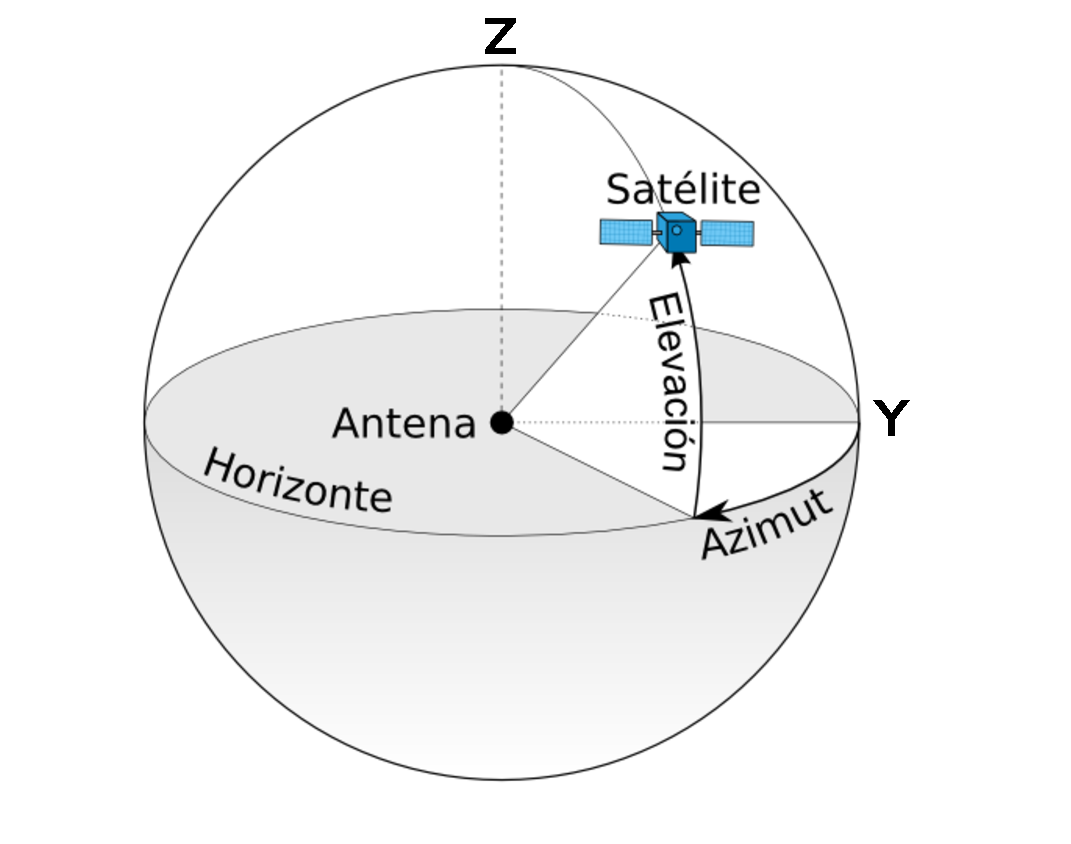
\includegraphics[width=0.55\textwidth]{Contenido/Cuerpo/Capitulo3/Fig1.eps}
	\captionof{figure}{Angulo de azimuth}
	\label{fig:ModeloMat:Fig1}
\end{center}
El angulo de azimuth es la posición alrededor del horizonte, medida desde un punto de referencia como el norte verdadero o el sur
verdadero. Los movimientos de azimuth ocurren alrededor del eje Z (vertical).

La elevación es la distancia del objeto por encima o por debajo del horizonte (también conocida como altitud en aplicaciones de
astronomía y aeroespaciales). Los movimientos de elevación ocurren alrededor del eje Y.

Los movimientos de balanceo ocurren alrededor del eje X a medida que gira con los ejes Y y Z.\\
El control que se hace en la gimbal está dado por un motor con control de posición y una IMU (sensor inercial).Dicha gimbal esta
montada en la parte delantera del vehículo aéreo como se muestra en la siguiente figura.
\begin{center}
	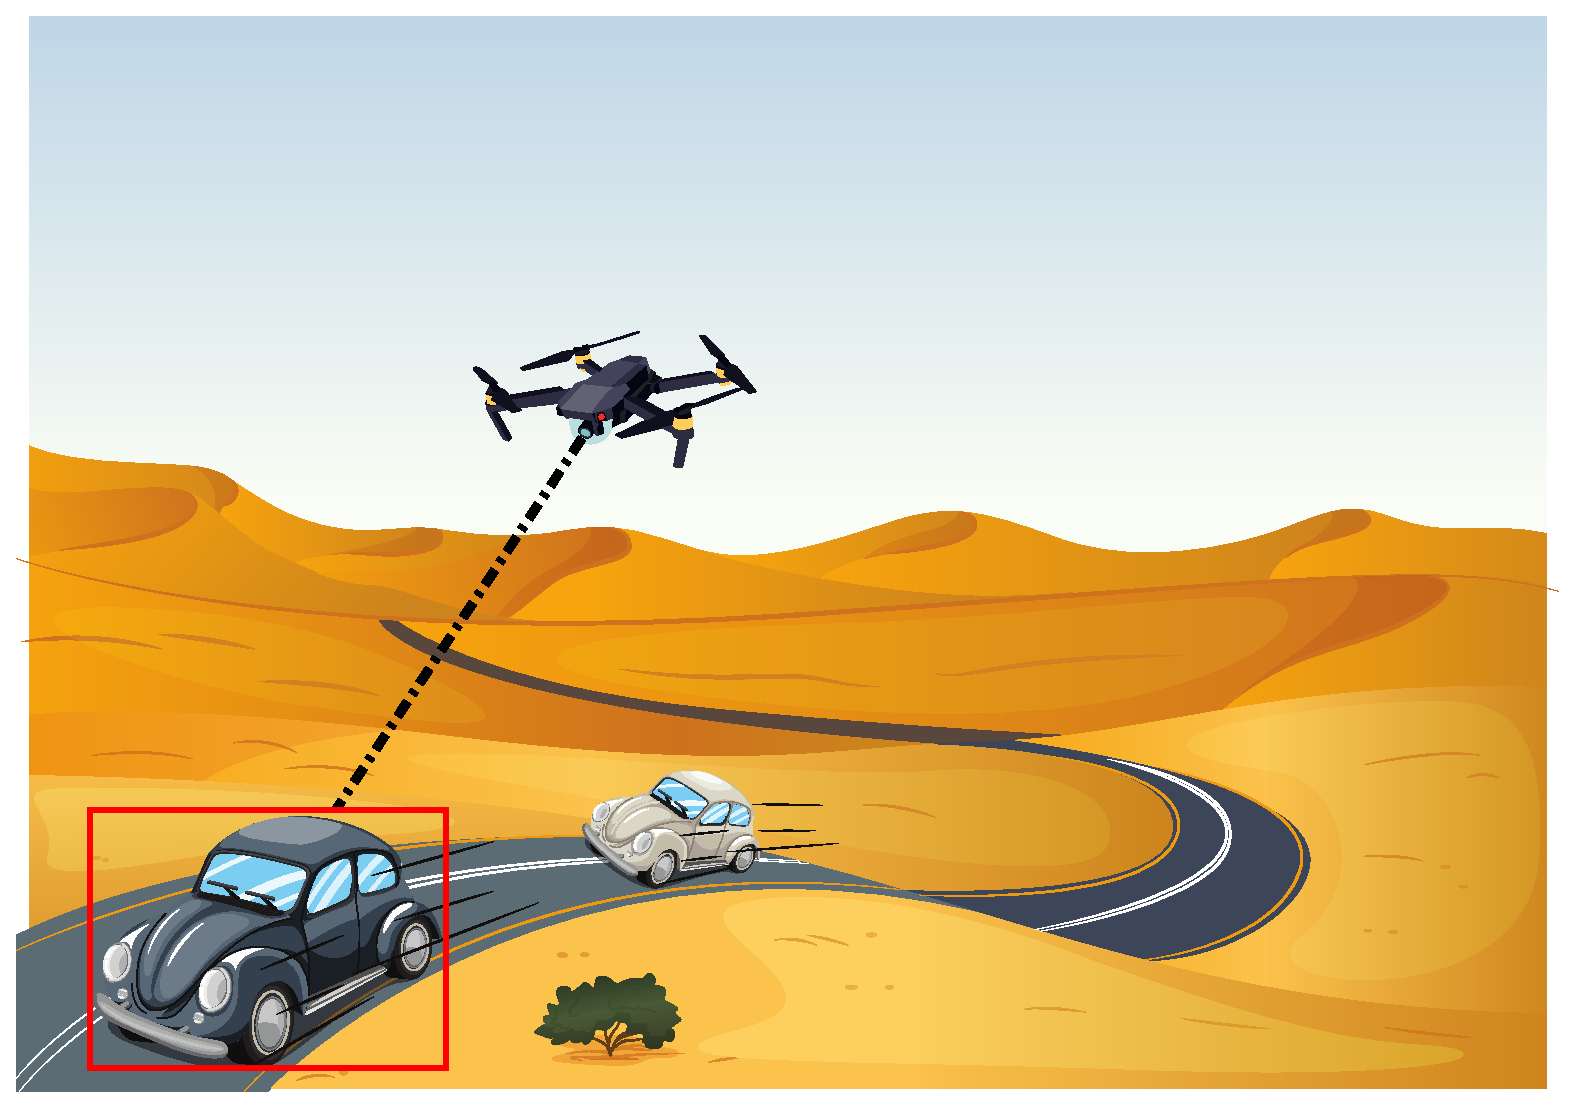
\includegraphics[width=0.55\textwidth]{Contenido/Cuerpo/Capitulo3/Fig2.eps}
	\captionof{figure}{Seguimiento de un objetivo utilizando una cámara sujeta a una gimbal embebida en un vehículo aéreo no tripulado.}
	\label{fig:ModeloMat:Fig1}
\end{center}

\subsection{Marco de referencia Inercial [I]}
Antes de abordar el control de la gimbal, es necesario y obvio conocer el comportamiento
de dicho sistema, empezaremos por definir el marco de referencia inercial, es decir
el de la tierra. La siguiente imagen ilustra los ejes de este marco.
\begin{center}
	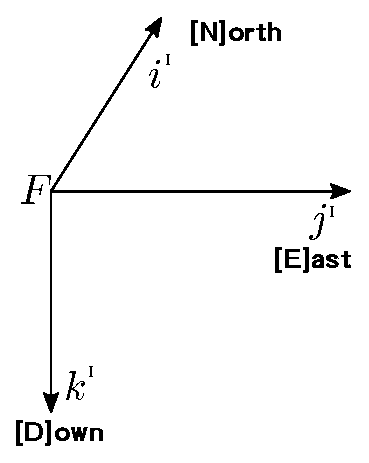
\includegraphics[width=0.25\textwidth]{Contenido/Cuerpo/Capitulo3/Fig4.eps}
	\captionof{figure}{Marco de referencia inercial}
	\label{fig:ModeloMat:Fig1}
\end{center}
Donde definimos a k apuntando hacia el centro de la tierra, este sistema de coordenadas
refieren a (Norte, Este y Abajo) de ahí su nombre NED(siglas en inglés).

\subsection{Marco de referencia del cuerpo [B]}
Una aeronave tiene la libertad de rotar en 3 ejes, en la aeronáutica son conocidos como
Yaw, Pitch y Roll. Dichas rotaciones son importantes en el control de aeronaves ya
que sirven para conocer la dinámica del sistema, dicha rotaciones pueden ser mejor
detalladas en una imagen, por lo que en la siguiente ilustración se grafica un plano
y se asigna nombre a cada rotación de los ejes.
\begin{center}
	
\includegraphics[width=0.35\textwidth]{Contenido/Cuerpo/Capitulo3/Fig6.eps}
	\captionof{figure}{Rotación en 3 ejes.}
	\label{fig:ModeloMat:Fig1}
\end{center}
Vamos a llamar marco de referencia del cuerpo a las coordenadas del UAV, es necesario establecer el centro del plano en el
centro de masas de la aeronave, como se ilustra en la siguiente figura.
\begin{center}
	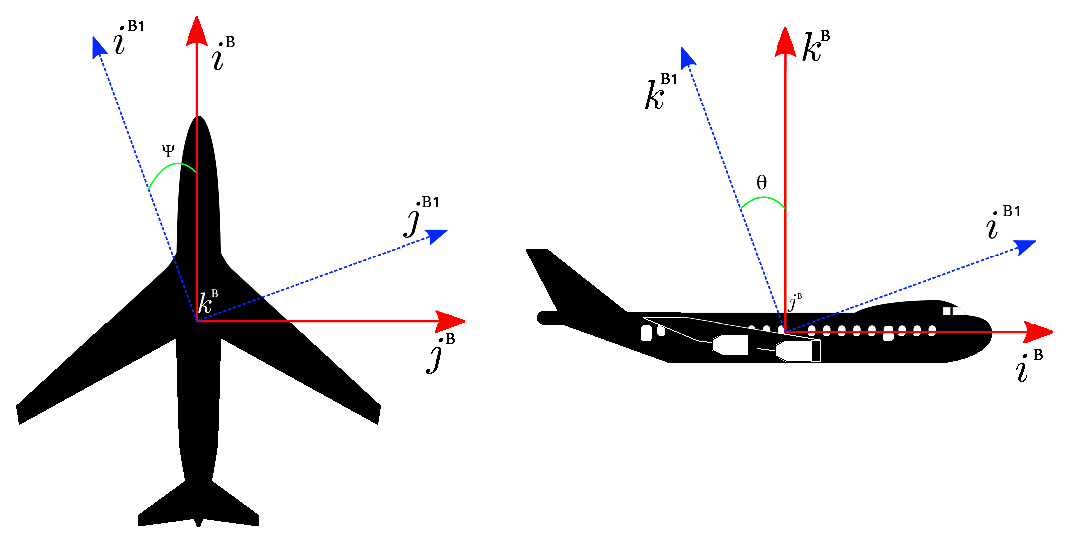
\includegraphics[width=0.5\textwidth]{Contenido/Cuerpo/Capitulo3/Fig5.eps}
	\captionof{figure}{Marco de referencia del cuerpo.}
	\label{fig:ModeloMat:Fig1}
\end{center}
De donde definimos las dos rotaciones que seran controladas en este trabajo pitch y yaw($\theta$, $\psi$). El subíndice B hace referencia
a Body y nos indica que estamos hablando de las coordenadas del UAV.

\subsection{Marco de referencia de la gimbal [G]}
Un último paso es definir un marco de referencia para la cámara, considerando que la cámara se encuentra en la parte delantera de
la aeronave y que el centro de la gimbal es el origen.
\begin{center}
	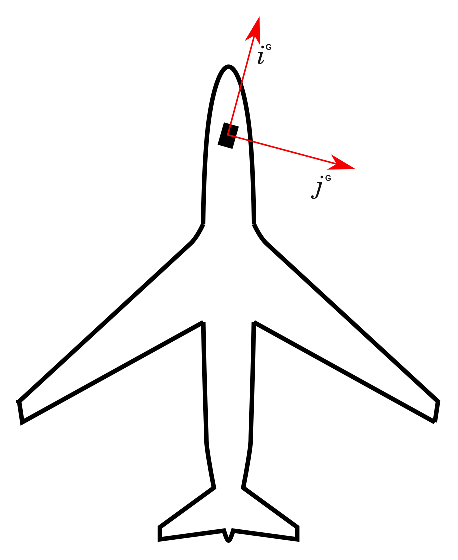
\includegraphics[width=0.3\textwidth]{Contenido/Cuerpo/Capitulo3/Fig7.eps}
	\captionof{figure}{Marco de referencia del la cámara.}
	\label{fig:ModeloMat:Fig1}
\end{center}
De donde el subíndice G hace referencia a que estamos en el plano de la gimbal. El vector unitario K apunta hacia afuera,
es decir hacia nosotros.


\section{Modelo matematico gimbal}
Poniendo en el mismo plano dos referencias, el de la gimbal y el del body, tal como se ilustra en la siguiente figura
\begin{center}
	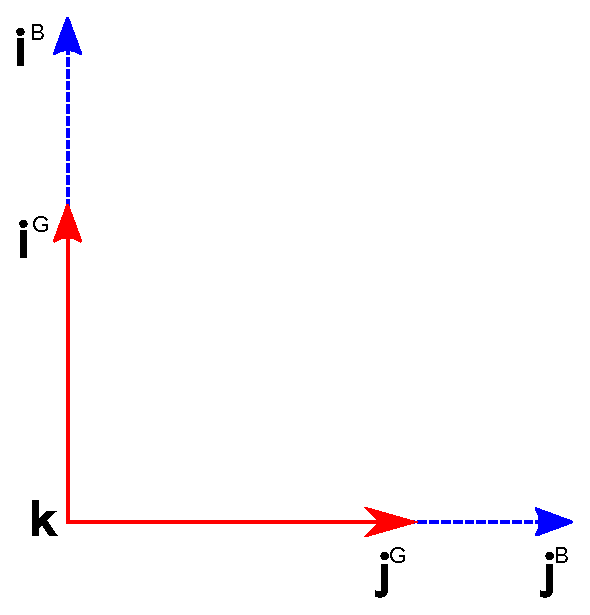
\includegraphics[width=0.3\textwidth]{Contenido/Cuerpo/Capitulo3/Fig8.eps}
	\captionof{figure}{Marco de referencia Body y gimbal}
	\label{fig:ModeloMat:Fig1}
\end{center}
Cualquier punto en el plano puede ser expresado como:
\begin{equation}
	p_{i^B,j^B} = [p_i^B , p_j^B]^T = p_i i^B + p_j p^B
\end{equation}
\begin{equation}
	p_{i^G,j^G} = [p_i^G , p_j^G]^T = p_i \cdot i^G + p_j\cdot  p^G
\end{equation}
\begin{equation}
	\textbf{P}_{i,j}^B = \textbf{P}_{i,j}^G
\end{equation}

Si hacemos rotar el frame de la gimbal respecto al eje K obtenemos que:
\begin{center}
	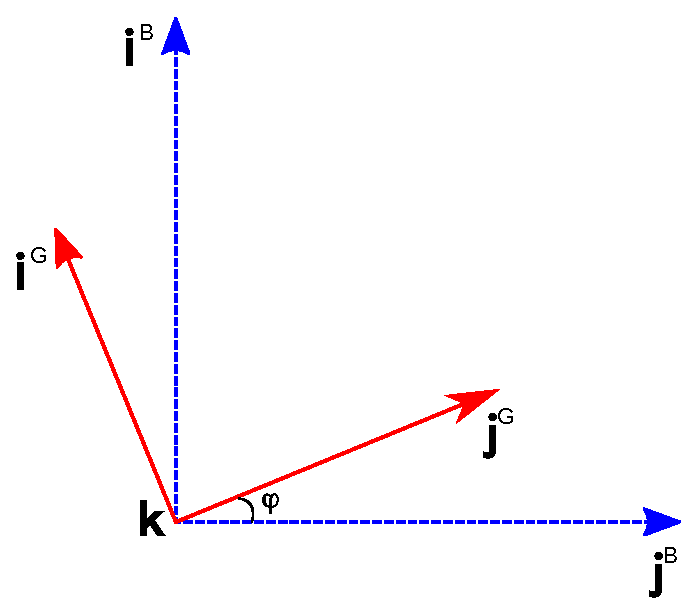
\includegraphics[width=0.3\textwidth]{Contenido/Cuerpo/Capitulo3/Fig9.eps}
	\captionof{figure}{Rotación del marco de referencia Gimbal respecto al del cuerpo}
	\label{fig:ModeloMat:Fig1}
\end{center}
\begin{equation}
	p_{i^B,j^B} = [p_i^B , p_j^B]^T = p_i i^B + p_j p^B
\end{equation}
\begin{equation}
	p_{i^G,j^G} = [p_i^G , p_j^G]^T = p_i i^G + p_j p^G
\end{equation}
Como
\begin{equation}
	p_i = p_{i,j}^G \cdot i^B = p_i^G i^B \cdot i^G + p_j^G i^B \cdot j^G
\end{equation}
\begin{equation}
	p_j = p_{i,j}^G \cdot j^B = p_i^G j^B \cdot i^G + p_j^G j^B \cdot j^G
\end{equation}
Entonces
\begin{equation*}
	\begin{bmatrix}
		p_i^B \\
		p_j^B
	\end{bmatrix}
	=
	R
	\begin{bmatrix}
		p_i^G \\
		p_j^G
	\end{bmatrix}
\end{equation*}
Donde la matriz de rotación etsa dada por:
\begin{equation*}
	R=
	\begin{bmatrix}
		i^B\cdot i^G & i^B \cdot j^G\\
		j^B\cdot i^G & j^B \cdot j^G
	\end{bmatrix}
	=
	\begin{bmatrix}
		cos(\psi) & -sin(\psi)\\
		sin(\psi) & cos(\psi)
	\end{bmatrix}
\end{equation*}